\clearpage
\section{Predictive Analysis}
\label{sec:predictive_analysis}

Our task is to forecast demand and availability in Leipzig in varying spatial and temporal resolutions.
% We define these areas as h3 hexagons.  
% Initially, we decided to make forecasts for hexagons of resolutions 7, 8 and 9, which measures are shown in the table X. However, with resolution 9 we had to restrict the time period to X due to large amount of data and not sophisticated computational power.

To accomplish this task we use three different models, which we will compare afterwards in terms of predictive performance and training speed.
The three models are a Support Vector Machine, XGBoost and Neural Network.

Our training approach is split into two main stages.
First, we perform hyper-parameter tuning for each model and outcome pair with a fixed spatial and temporal resolution. Then, we will use the best hyper-parameters obtained from the tuning to fit models for varying temporal and spatial resolutions.
To ensure that no data leakage occurs we split our data into training and test split before any hyper-parameter tuning and we will only use the test to evaluate the performance of our final models.
Lastly, we can compare the two model types and evaluate how differing the spatial and temporal resolution impacts the predictive performance.


Our approach for the hyper-parameter tuning differs for the Neural Network and the Support Vector Machine.

For the Neural Network we employ a multi-staged grid search, where we try to find a subset of hyper-parameters in one stage and then use the best performing setting for these hyper-parameters in the consecutive stages.
While this approach does not guarantee to find the optimal hyper-parameters, a full scale grid search would be computationally intractable and we expect that our approach will result in a reasonable approximation.
To avoid reduce training time, avoid overfitting and ensure that the model is sufficiently trained we will use a high number of epochs and stop the model when the validation loss does not decrease any further in all stages.
% explain early stopping?
In the first stage we will find the best batch size by training multiple instances of a simple single-layer Neural Network, where the number of nodes are equal to the number of input features.
In the second stage we will find the best architecture of the model by performing a grid search on various number of layers, nodes as well as the two common hidden activation functions, namely the rectified linear unit and the hyperbolic tangent.
In the third stage we try to improve the generalizability by implementing regularization through dropout layers.
We add dropout layers after every hidden layer and vary the dropout rates between 0 (no dropout) and 0.5 (dropout nodes half of the time).

For the Support Vector Machines we perform three separate grid searches for a linear, polynomial and radial function kernel (RBF), respectively.
This way we are able to compare the different kernels in predictive performance, as well as, training time.
% kfold!!!
In order to speed up the grid search we employ a grid search with successive halving.
Grid search with successive halving first evaluates all candidates (combinations of hyper-parameter settings) with a small fraction of the training set.
After completion the best performing one third of all candidates get trained again on a fraction of the dataset that is three times as big as in the previous stage.
This repeats until only a few of the  best performing candidates get evaluated on the whole dataset.
After that the best hyper-parameter combination is chosen.
This approach achieves similar results to a full scale grid search, while being much faster. (citation Non-stochastic Best Arm Identification and Hyperparameter Optimization
Kevin Jamieson, Ameet Talwalkar).

For all three kernels we use various values on a log scale for the regularization parameter \(C\).
The regularization parameter determines the weight of a regularization term in the loss function that tries to minimize the coefficients of model.
For the RBF kernel we will also use different values for the bandwidth \(gamma\), also on a log scale.
The bandwidth \(gamma\) determines how large the influence of a single sample is on predictions made near to it.
For the polynomial kernel we will vary the degree, which determines the degree of the polynomial that is used to (pseudo) project the data into a higher dimensional space.

For XGBoost, we perform a hyper-parameter search based successive halving, similar to our approach applied to SVMs.
However, in comparison to SVM, where we applied successive halving to a predefined hyper-parameter grid, this time we will only specify distributions for the (continuous) hyper-parameters and sample from these distributions in a randomized fashion.
Randomized search has multiple advantages compared to grid search.
First we do not have to create an explicit hyper-parameter grid with discrete values, but instead we can define distributions. Second, we can easily increase or decrease the amount of models that we want to try, without altering the specification of the grid. Third, randomized searches are more efficient that grid searches \shortcite{bergstra}.
Kein erklärung von XGBoost hyper-parameters (haben wir dafür wirklich platz)?


% Hier sind Referenzen zu den papern, die das erfunden haben
% https://scikit-learn.org/stable/modules/grid_search.html#id3
\begin{figure}
    \centering
    \begin{minipage}{.5\textwidth}
        \centering
        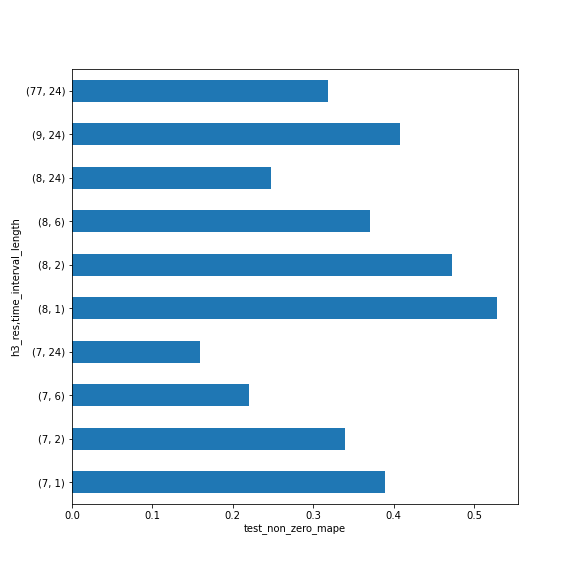
\includegraphics[width=\linewidth]{figures/predictive_analysis/demand_test_non_zero_mape.png}
        \captionof{figure}{Non-zero MAPE - Demand}
        \label{fig:non_zero_mape_demand}
    \end{minipage}%
    \begin{minipage}{.5\textwidth}
        \centering
        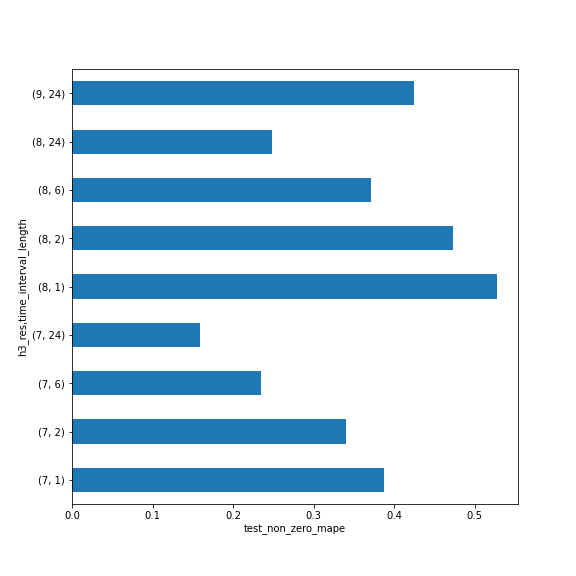
\includegraphics[width=\linewidth]{figures/predictive_analysis/availability_test_non_zero_mape.png}
        \captionof{figure}{Non-zero MAPE - Availability}
        \label{fig:non_zero_mape_availability}
    \end{minipage}
\end{figure}




\begin{figure}
    \centering
    \begin{minipage}{.4\textwidth}
        \centering
        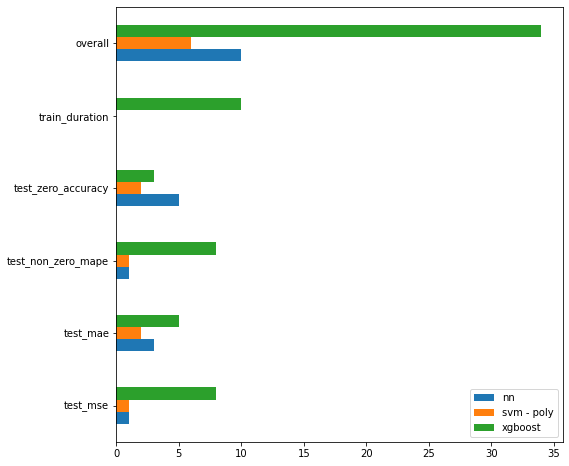
\includegraphics[width=\linewidth]{figures/predictive_analysis/demand_benchmark.png}
        \captionof{figure}{Prediction Models Benchmark - Demand}
        \label{fig:prediction_models_benchmark_demand}
    \end{minipage}%
    \begin{minipage}{.4\textwidth}
        \centering
        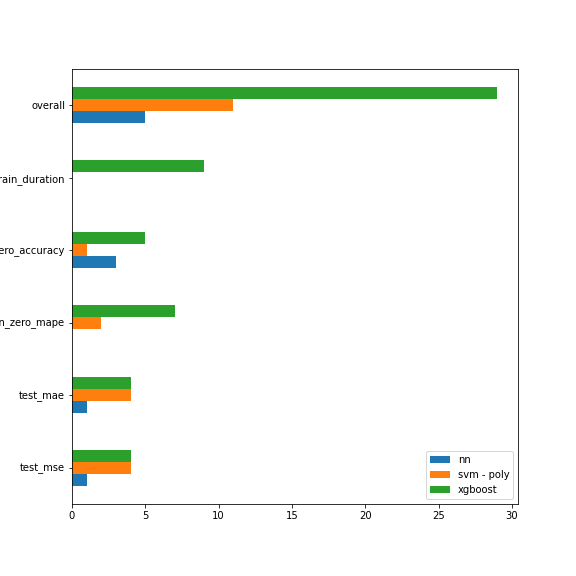
\includegraphics[width=\linewidth]{figures/predictive_analysis/availability_benchmark.png}
        \captionof{figure}{Prediction Models Benchmark - Availability}
        \label{fig:prediction_models_benchmark_availability}
    \end{minipage}
\end{figure}




% alter text 
%We decided to build multiple Support Vector Machine (SVM) models with linear, polynomial and rbf kernels, thus covering multiple functional forms. We also opted for a multitude of neural networks with different architectures to capture more complex relationships.
%Brute force search of hyperparameters ...
%K-fold validation
%In total we have trained X svm models and X neural networks. Table X shows are top 10 best performing models and their respective test metrics.








% Mo's text backup friday 08.07
% Our task is to forecast demand and availability in Leipzig with varying spatial and temporal resolutions.
% % We define these areas as h3 hexagons.  
% % Initially, we decided to make forecasts for hexagons of resolutions 7, 8 and 9, which measures are shown in the table X. However, with resolution 9 we had to restrict the time period to X due to large amount of data and not sophisticated computational power.

% To accomplish this task we use three different models, which we will compare afterwards in terms of predictive performance and training speed. 
% The three models are a Support Vector Machine, XGBoost and Neural Network.  

% Our training approach is split into two main stages.
% First, we perform hyper-parameter tuning for each model and outcome pair with a fixed spatial and temporal resolution. Then, we will use the best hyper-parameters obtained from the tuning to fit models for varying temporal and spatial resolutions.
% To ensure that no data leakage occurs we split our data into training and test split before any hyper-parameter tuning and we will only use the test to evaluate the performance of our final models.
% Lastly, we can compare the two model types and evaluate how differing the spatial and temporal resolution impacts the predictive performance.  


% Our approach for the hyper-parameter tuning differs for the Neural Network and the Support Vector Machine. 

% For the Neural Network we employ a multi-staged grid search, where we try to find a subset of hyper-parameters in one stage and then use the best performing setting for these hyper-parameters in the consecutive stages.
% While this approach does not guarantee to find the optimal hyper-parameters, a full scale grid search would be computationally intractable and we expect that our approach will result in a reasonable approximation.
% To avoid reduce training time, avoid overfitting and ensure that the model is sufficiently trained we will use a high number of epochs and stop the model when the validation loss does not decrease any further in all stages.
% % explain early stopping?
% In the first stage we will find the best batch size by training multiple instances of a simple single-layer Neural Network, where the number of nodes are equal to the number of input features.
% In the second stage we will find the best architecture of the model by performing a grid search on various number of layers, nodes as well as the two common hidden activation functions, namely the rectified linear unit and the hyperbolic tangent.
% In the third stage we try to improve the generalizability by implementing regularization through dropout layers.
% We add dropout layers after every hidden layer and vary the dropout rates between 0 (no dropout) and 0.5 (dropout nodes half of the time).

% For the Support Vector Machines we perform three separate grid searches for a linear, polynomial and radial function kernel (RBF), respectively.
% This way we are able to compare the different kernels in predictive performance, as well as, training time.
% % kfold!!!
% In order to speed up the grid search we employ a grid search with successive halving. 
% Grid search with successive halving first evaluates all candidates (combinations of hyper-parameter settings) with a small fraction of the training set.
% After completion the best performing one third of all candidates get trained again on a fraction of the dataset that is three times as big as in the previous stage.
% This repeats until only a few of the  best performing candidates get evaluated on the whole dataset.
% After that the best hyper-parameter combination is chosen.
% This approach achieves similar results to a full scale grid search, while being much faster. (citation Non-stochastic Best Arm Identification and Hyperparameter Optimization
% Kevin Jamieson, Ameet Talwalkar).

% For all three kernels we use various values on a log scale for the regularization parameter \(C\).
% The regularization parameter determines the weight of a regularization term in the loss function that tries to minimize the coefficients of model.
% For the RBF kernel we will also use different values for the bandwidth \(gamma\), also on a log scale.
% The bandwidth \(gamma\) determines how large the influence of a single sample is on predictions made near to it.
% For the polynomial kernel we will vary the degree, which determines the degree of the polynomial that is used to (pseudo) project the data into a higher dimensional space.  

% For XGBoost, we perform a hyper-parameter search based successive halving, similar to our approach applied to SVMs. 
% However, in comparison to SVM, where we applied successive halving to a predefined hyper-parameter grid, this time we will only specify distributions for the (continuous) hyper-parameters and sample from these distributions in a randomized fashion.
% Randomized search has multiple advantages compared to grid search.
% First we do not have to create an explicit hyper-parameter grid with discrete values, but instead we can define distributions. Second, we can easily increase or decrease the amount of models that we want to try, without altering the specification of the grid. Third, randomized searches are more efficient that grid searches \shortcite{bergstra}.
% Kein erklärung von XGBoost hyper-parameters (haben wir dafür wirklich platz)?
